\chapter{Estado del Arte}\label{chapter03}

Según \parencite{creswell2014}, el estado del arte constituye una instancia fundamental dentro del proceso de investigación debido a que permite conocer las soluciones vigentes a la problemática abordada, identificar los aportes realizados por otros actores y a su vez delimitar las distintas oportunidades de innovación para el proyecto en curso.

En este sentido, el presente apartado desarrolla un análisis del estado del arte en relación con el diseño de soluciones tecnológicas orientadas a la gestión inteligente del stock en el sector gastronómico, haciendo énfasis en aplicaciones que incorporan técnicas de \emph{Machine Learning} para la predicción de la demanda.

Ahora bien, con el objetivo de identificar los aportes diferenciales de la solución propuesta, se abordan tres tópicos esenciales: primeramente aplicaciones comerciales actuales, en segundo lugar proyectos académicos o experimentales relacionados, y por último una lectura estratégica basada en la teoría del Océano Azul para identificar oportunidades de innovación y creación de valor en espacios de mercado poco explorados.

\section{Soluciones tecnológicas con enfoque predictivo en el sector gastronómico internacional}\label{sec:estado-internacional}

A nivel mundial, la búsqueda por una gestión eficiente de los establecimientos gastronómicos ha impulsado el desarrollo de herramientas que integran inteligencia artificial, especialmente técnicas de Machine Learning. Estas soluciones han surgido en distintos países con el objetivo de anticipar la demanda y optimizar la administración de insumos. A continuación, se presentan dos de las plataformas más relevantes, con el fin de profundizar en el uso de la inteligencia artificial en el sector gastronómico a nivel global.

\begin{itemize}
    \item \textbf{5-Out}. Plataforma estadounidense que utiliza \emph{Machine Learning} para predecir ventas con integración de fuentes internas (TPV, programación de personal, reservas) y externas (clima, eventos), habilitando recomendaciones de compra para equilibrar inventario y reducir desperdicio. Es integrable con sistemas como Toast, Square y 7Shifts; además, anunció una alianza con Craftable para ampliar funciones administrativas y financieras \parencite{fiveout2025partnership}.

        Gracias al análisis predictivo, esta herramienta puede indicarle de forma detallada al sitio gastronómico la cantidad de productos que deberá comprar para mantener un equilibrio en la gestión del inventario. Esto ayuda a reducir significativamente el desperdicio de alimentos y aumenta en consecuencia la rentabilidad. 

        Además, esta aplicación es compatible e integrable a sistemas actuales como Toast, Square y 7Shifts, y consideran unirse a Craftable para sumar funciones administrativas y financieras a sus capacidades predictivas como alternativa innovadora en la gestión de restaurantes. 

    \item \textbf{Restoke}. Es una startup australiana que automatiza procesos administrativos en restaurantes mediante IA: control de inventario y compras, programación y proyección de ventas, e integración con POS y software contable. En 2024 fue noticia por su crecimiento y una ronda de financiación de USD 5,1 millones, con casos reportados de fuertes reducciones de costos operativos \parencite{santoreneos2024restoke}.
\end{itemize}

\subsection{Soluciones comerciales actuales en el sector gastronómico argentino}\label{sec:estado-arg}

Actualmente, en Argentina, el mercado del software especializado en el sector gastronómico se encuentra en constante crecimiento, que si bien todavía no ha explotado el mundo del aprendizaje automatizado, dispone de herramientas que facilitan la administración y operación diaria de distintos establecimientos como restaurantes, sitios de comida rápida, cafés y lugares afines. Es por esto que se resalta algunas de las plataformas más utilizadas dentro del presente rubro, Maxirest y Restô , ambas con un enfoque integral en la gestión del negocio.

\begin{itemize}
    \item \textbf{Maxirest} \parencite{latam2024maxirest}. Se trata de una herramienta reconocida en el mercado por su robustez y funcionalidad. Su enfoque se centra exclusivamente en el análisis descriptivo de datos históricos y es una de las soluciones más consolidadas del país en el ámbito gastronómico. La plataforma permite automatizar diversas tareas operativas, tales como la gestión de cocina, la toma de pedidos, la administración de reservas e inventario, y la generación automática de reportes. Además, incluye un módulo específico para delivery y takeaway, lo que resulta especialmente relevante considerando que el 47,6\% de las ventas del sector se realizan a través de estas dos modalidades.
    
    \item \textbf{Restô} \parencite{iprofesional2014resto}. Es un sistema de gestión gastronómica que forma parte del ecosistema del software Tango, el cual fue desarrollado por la empresa argentina Axoft. El propósito de este es brindar una solución a la necesidad de una herramienta tecnológica que simplifique los procesos del día a día de dicho sector. En línea con dicho objetivo, este brinda una administración integral en múltiples establecimientos gastronómicos con diversas funciones tales como la gestión de mesas y reservas, el control de stock de insumos, la facturación electrónica, el seguimiento de ventas, y muchas otras más. De igual manera, gracias a su enfoque modular y adaptable, es utilizado tanto por pequeños comercios como por grandes cadenas gastronómicas, lo que le ha permitido posicionarse como una de las soluciones locales más completas del mercado para la administración de negocios del rubro alimenticio.
\end{itemize}

\subsection{Propuestas académicas y experimentales}\label{sec:academico}

Aunque el modelo predictivo se ha desarrollado en investigaciones de múltiples áreas, existen escasos trabajos académicos enfocados específicamente en el rubro gastronómico. Uno de ellos es \parencite{hari2024predictiwaste}: \emph{PredictiWaste: An ML-Powered Framework for Sustainable Food Inventory Optimization in Restaurants (marco de trabajo basado en aprendizaje automático para la optimización sostenible del inventario de alimentos en restaurantes)}, se introduce un modelo de análisis predictivo para reducir el desperdicio de alimentos en el inventario y la planificación de menús de restaurantes. 

Por consiguiente, realiza el pronóstico del desperdicio basándose en factores como el tipo y cantidad de alimento, número de comensales, tipo de evento, condiciones de almacenamiento, historial de compras, métodos de preparación, estacionalidad, ubicación y precio. El sistema clasifica el desecho como mínimo, moderado o alto y sugiere medidas de control de inventario, ayudando en consecuencia a las empresas a optimizar sus recursos y a promover la sostenibilidad. 

Igualmente, una de las propuestas más representativas se encuentra en \parencite{schmidt2022mlsales}, con el pronóstico de ventas de restaurantes basado en aprendizaje automático. Este estudio afirma que para la correcta gestión del personal en los restaurantes, es necesaria la previsión precisa de las ventas, y propone un caso práctico sobre diversos modelos de aprendizaje automático utilizando data real de las ventas de un negocio, tipo restaurante de tamaño medio, y la inclusión de modelos de redes neuronales recurrentes de tendencia para la comparación de su rendimiento a través de diversos métodos.

De la misma manera, otros estudios como el \parencite{tanizaki2019forecasting} sobre la previsión de la demanda en restaurantes mediante aprendizaje automático y análisis estadístico, construyen un modelo específico para cada tienda física que combina funcionalmente datos de diversos factores externos tales como ubicación, clima y eventos, mediante aprendizaje automático, para luego analizar el resultado de verificación con datos de otros negocios similares.

\subsection{Océano Azul}

La Estrategia del Océano Azul es una teoría innovadora conceptualizada en \parencite{kim2015estrategia} que redefine la competencia empresarial a través de la innovación, como creadora de oportunidades y crecimiento rentable en mercados inexplorados.

Según sus autores, los océanos rojos representan a todas las industrias que hoy operan en el mercado, donde sus características están altamente definidas y son aceptadas, lo que conlleva a la lucha entre empresas rivales por obtener el posicionamiento ventajoso de llevarse una mayor participación en la demanda existente. Es decir, es un nivel de subsistencia toda vez que al saturarse el mercado se reducen las perspectivas de rentabilidad y sostenibilidad, lo que ocasiona que los productos pierdan su rasgo de distinción y por ende se conviertan en genéricos.

Por el contrario, los océanos azules representan nichos de mercado no explorados donde es factible la creación de demanda con un crecimiento altamente rentable. En el contexto de los océanos azules, la competencia carece de relevancia, dado que los parámetros operativos aún no han sido definidos.

Los teóricos con la intención de cuantificar el impacto de la creación de los océanos azules sobre el crecimiento de una compañía, analizaron el lanzamiento de 108 negocios nuevos, lo que arrojó como resultado que el 86\% eran extensiones de líneas existentes, es decir, pertenecientes al océano rojo y el 14\% restante de los lanzamientos pertenecientes a océanos azules.

Esto subraya la diferencia entre la creación de nuevos mercados sin competencia que rompen el equilibrio tradicional entre valor y costos, generando crecimiento empresarial con ganancias más rentables y a su vez con la competencia tradicional directa en mercados ya existentes que se encuentran saturados por parte de empresas que luchan por el control de la demanda.

En la estrategia del océano azul, se definen como varias herramientas fundamentales a saber, la matriz de \emph{Eliminar-Reducir-Aumentar-Crear} como recurso central, que \guillemotleft obliga a las compañías no solo a perseguir simultáneamente la diferenciación y el bajo costo, sino también a romper con el compromiso de valor-costo. No se trata de crear una nueva curva de valor por crearla, sino de identificar las variables correctas que transformarán la dinámica de la industria.\guillemotright \parencite{kim2015estrategia}.

Este enfoque analítico desafía la lógica de la competencia tradicional de la industria brindando apertura a nuevos paradigmas de análisis económico, ya que impulsa a las empresas a pensar de manera diferente sobre cómo crear valor para el cliente. 

Ahora bien, la Matriz \emph{Eliminar-Reducir-Aumentar-Crear}, es la representación tabular del Marco de las Cuatro Acciones, y tiene como finalidad ayudar en la formación de las ideas para que la toma de decisiones tenga como objetivo la diferenciación y el bajo costo de manera integrada.

Asimismo, otra herramienta fundamental es la \emph{Curva de Valor}, la cual permite una visualización gráfica del perfil estratégico de una empresa en relación con los factores clave de la industria. Esta curva permite identificar si una propuesta se encuentra alejada o no, de lo convencional, permitiendo así la detección temprana de oportunidades de innovación que generen una ventaja competitiva sostenible dentro del mercado.


\subsection{Matriz ERAC}\label{sec:erac}

\begin{figure}[htbp]
    \centering
    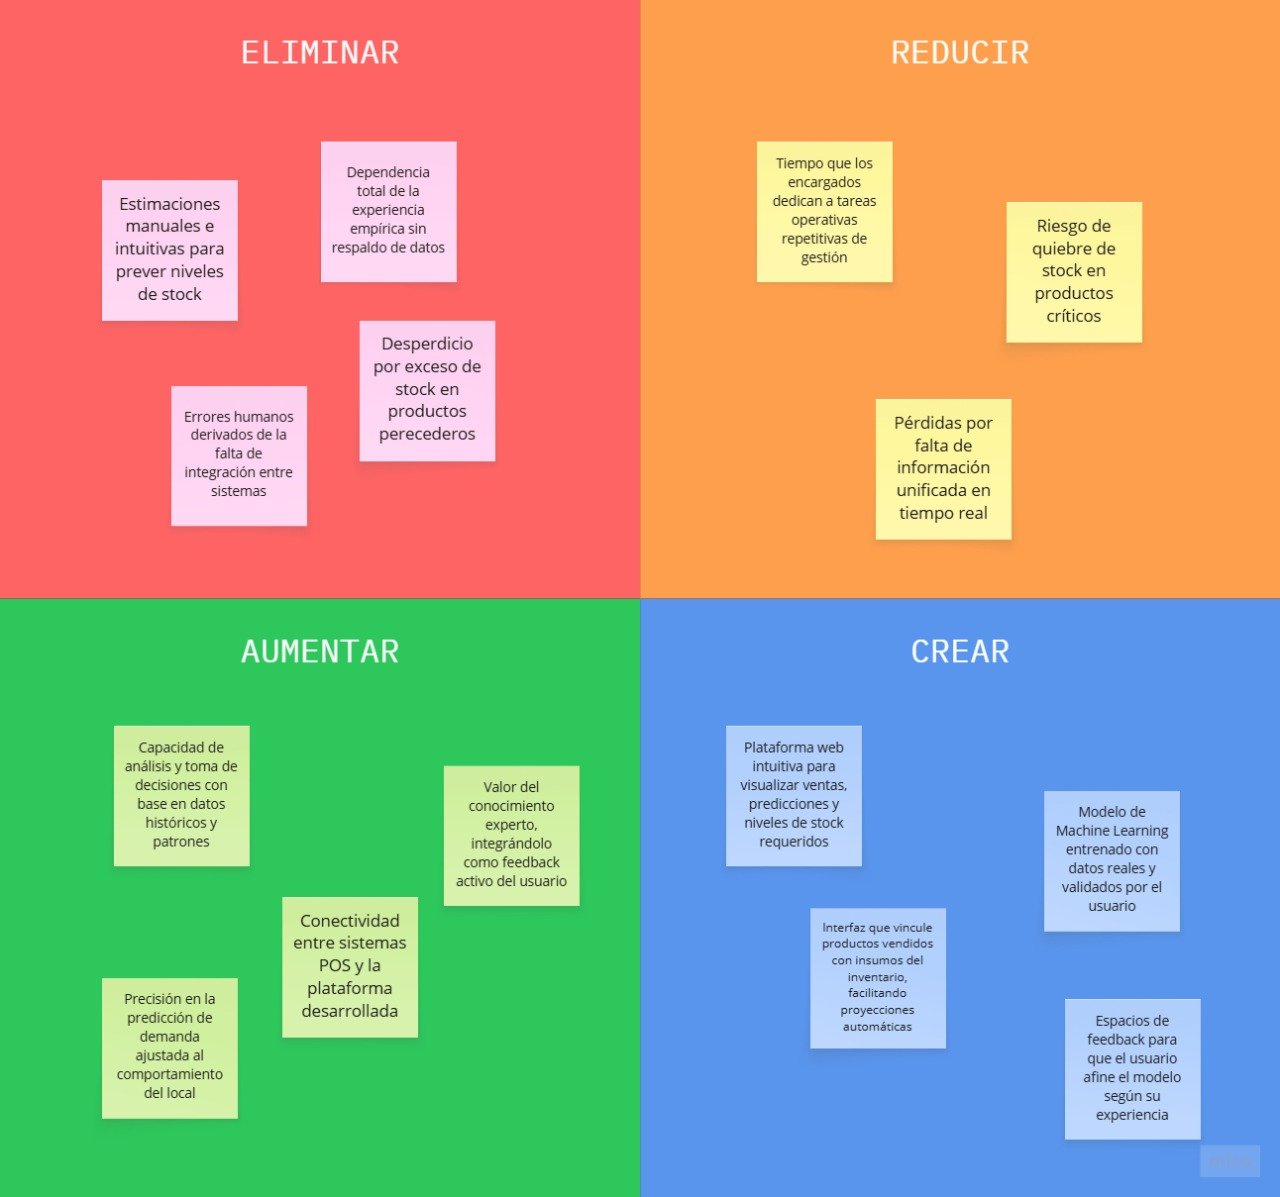
\includegraphics[width=0.7\textwidth]{images/matrizEric.jpeg}
    \caption{Matriz ERAC de SmartStocker}
    \label{fig:eric}
\end{figure}

Las variables identificadas en la matriz ERAC (Fig.~\ref{fig:eric}) se utilizan como insumo para construir la Curva de Valor (Fig.~\ref{fig:curva}), con el objetivo de visualizar el posicionamiento de \emph{SmartStocker} en relación con sus competidores en el mercado.

\FloatBarrier

\clearpage
\subsection{Curva de Valor}\label{sec:curva-valor}

\begin{figure}[htbp]
    \centering
    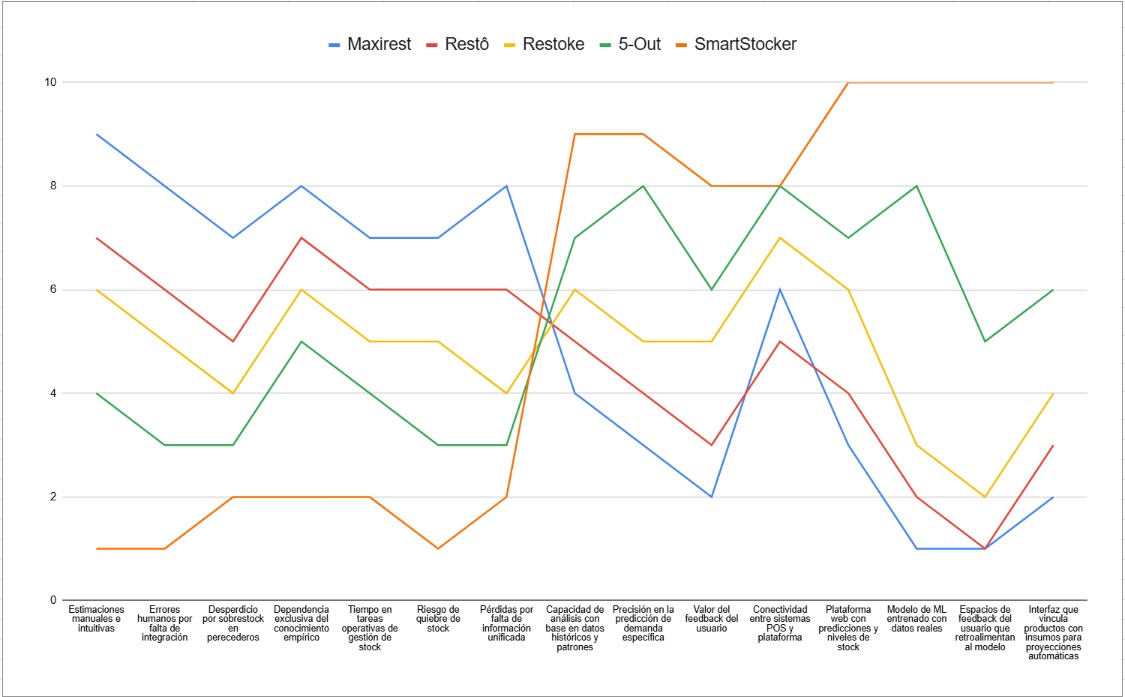
\includegraphics[width=0.7\textwidth]{images/curvaValor.jpeg}
    \caption{Curva de valor}
    \label{fig:curva}
\end{figure}

\FloatBarrier

\subsection{Síntesis}\label{sec:sintesis-estado}

Una vez realizado el análisis del estado del arte y de las herramientas que utiliza, se evidencia el diferencial del presente proyecto ya que no existen en la actualidad soluciones tecnológicas predictivas en el mercado nacional que conduzcan a una precisa gestión del inventario en el rubro gastronómico en base a la información de ventas, toda vez que las otras plataformas en el mercado se limitan a funciones descriptivas, basadas en estadísticas generales de consumo.

Asimismo, la presente tesis desarrolla un enfoque novedoso ya que utiliza el modelo de Machine Learning para predecir las cantidades de producto necesarias para el funcionamiento óptimo del usuario, ajustar los niveles de existencias en tiempo real y mantener los niveles de stock necesarios para que el local sea altamente productivo y su rentabilidad sea sostenible.

Mantener el inventario en un punto de equilibrio óptimo impacta directamente en la eficiencia operativa del negocio ya que implica la reducción de costos y la posibilidad de minimizar el capital inactivo en productos consumibles. Como consecuencia, genera grandes beneficios tales como el control de los desperdicios que puede traducirse a corto plazo en una reducción de gastos. Permite la rotación correcta de los insumos, evita la sobrecompra y la posible merma por caducidad ya que los alimentos tienen un tiempo de vida útil limitado, y luego de transcurrido este, no queda otra que descartarlos por control sanitario. Consecuencialmente, también se evita el gasto colateral que se genera en tiempo horas-hombre en personal utilizado para eliminar desechos, asear y reacondicionar el lugar.

Además, permite determinar el stock de seguridad, lo que es igual a la cantidad mínima de insumos necesarios para la producción base del negocio, facilitando así la gestión de mantenimiento de los volúmenes necesarios con el fin de evitar posibles rupturas en la cadena de suministro, ya que puede establecerse de manera certera el punto de pedido en el que es necesario emitir una orden de compra. 

Cabe resaltar que un exceso en los niveles de inventario es negativo para negocios con espacios limitados lo que puede conllevar al inadecuado uso de algunos productos con fecha cercana a la caducidad como medida de aprovechamiento de la materia prima, esto disminuye el nivel del servicio y por ende la competitividad del negocio.

En consecuencia, favorece la gestión de compras, evitando la adquisición urgente de materiales específicos necesarios para la elaboración de platos, por lo que asegura la disponibilidad constante de insumos para la totalidad del menú y garantiza la integridad de la oferta gastronómica, que es la principal fuente de ingresos del usuario. Evita además cambios abruptos en los stocks que podrían afectar el nivel de servicio como elemento esencial y diferenciador de la competencia y que además conforman una parte importante de los lineamientos estratégicos de la empresa para que su productividad sea sostenible.  

Dada la inexistencia de un sistema de gestión de stocks con un modelo predictivo en base a la información de ventas, el presente trabajo es una herramienta innovadora en el área gastronómica para aquellos negocios que desean aumentar su capacidad de  producción a través del manejo eficiente de su reabastecimiento.

Por otro lado, uno de los factores más importantes del costo de las operaciones empresariales está relacionado con el capital  invertido en la reposición de inventario necesario para el funcionamiento del local, el cual al quedar cautivo anula cualquier posibilidad de reinversión directa o de un nuevo destino generador de rentabilidad y posicionamiento.

En esta medida, dada la inmovilidad del capital, es determinante tomar decisiones que reduzcan costos, con lo cual surge la necesidad de regular los niveles de stock de los productos, cuantificarlos y gestionar su reposición. Aunque los inventarios almacenan valor, pueden generar una pérdida irrecuperable para el usuario cuando hay sobreabastecimiento, todo esto debido a que absorben el capital que podría estar disponible para otras opciones de inversión, sin embargo, lo paralizan y hasta pueden generar pérdidas cuando los consumibles se vencen o deterioran. También es importante la administración del espacio, ya que un stock superior al que puede ser preservado o refrigerado puede deteriorar sus componentes y por ende se podría ver afectada la calidad del producto final.

En otro sentido, disponer de pocos insumos genera una pausa considerable en la producción y  desmejora la calidad del producto ofrecido en el menú, lo que podría traducirse en el aumento de los costos por la carencia de artículos en el momento de ser demandados, pérdida de los beneficios originados de la venta imposible y el deterioro de la imagen comercial de la empresa, impulsando finalmente al consumidor a adquirir el bien a través de la competencia. Esta negativa también está asociada con la demora a la hora de satisfacer la demanda de pedidos al  momento en que son solicitados. 

Por otro lado, debe considerarse el análisis de la ventas como un factor fundamental para determinar la logística que deberá emplear la empresa para la reposición de inventario y así establecer su modelo de gestión. La predictibilidad entonces estará determinada por elementos probables y no por factores aleatorios, ya que la toma de decisiones se hará en función de estadísticas fidedignas arrojadas por el sistema alimentado con datos actualizados proporcionados por el usuario.

En consecuencia, la solución propuesta en esta tesis sobre la optimización de los niveles de stock en el rubro gastronómico de Argentina en el año 2025, utilizando modelos de Machine Learning para predecir los niveles requeridos en base a la información de ventas, resulta técnicamente factible y presenta un concepto innovador en gestión empresarial ya que pretende optimizar mecanismos de producción a través de la predictibilidad. Se configura en una herramienta avanzada para los propietarios de restaurantes y negocios afines, quienes a través de su implementación podrán obtener notables beneficios en cuanto a productividad y rentabilidad. Por último, el presente trabajo representa la oportunidad de crear un nuevo nicho de mercado en Argentina, específicamente la Ciudad Autónoma de Buenos Aires, basado en la innovación tecnológica por medio de la toma de decisiones informadas sustentadas en estadísticas proporcionadas por el mismo usuario.  


\section{User research}\label{sec:user-research}

\subsection{Entrevistas}\label{sec:entrevistas}

Durante la etapa de descubrimiento del proyecto se consideró fundamental realizar entrevistas cualitativas con el fin de comprender a profundidad las múltiples dificultades que se enfrentan actualmente en la administración de negocios gastronómicos, buscando indagar tanto en las dinámicas como en los patrones diarios dentro del sector, especialmente en la gestión de inventarios y su impacto sobre dichos negocios.

Primeramente se entrevistó a Ulises Litterio, dueño de La Brava Burguer, la cual es una cadena gastronómica que consta de tres locales y 25 empleados. Se centra en la venta de hamburguesas y llevan a cabo todas las actividades correspondientes para el mantenimiento y desarrollo de calidad de las mismas que van desde la compra de materias primas hasta la venta final de estas con delivery propio. Ahora bien, el control del inventario se encuentra descentralizado, básicamente cada jefe de cocina realiza un conteo el cual se le informa al encargado, quien lo carga en una planilla de Excel que luego es revisada por el dueño (Ulises Litterio). Además, todas las compras necesarias son realizadas de manera semanal, aunque pueden repetirse en distintos momentos de la semana si hay productos o ingredientes faltantes.

El cálculo de reposición de stock se basa en datos como las ventas semanas anteriores, fechas clave, como feriados, y la intuición de los trabajadores sobre la demanda esperada. Sin embargo, gestionar el inventario de esta manera conlleva una alta tasa de error tanto por sobrestock como por faltantes, lo cual genera desperdicios tanto a nivel económico como alimenticio. Además, Ulises destaca la dificultad de consolidar datos de ventas debido a que operan con múltiples plataformas de delivery como Rappi y PedidosYa, cada una con su propio sistema individual, y aunque ha considerado la opción de emplear un software como MaxiRest, ha terminado por descartar dicha idea debido a los costos elevados que tendría que pagar.

En segundo lugar, se entrevistó a Oscar Campione, dueño de una rotisería familiar que opera con un único local instalado en una parte de la casa. La venta del negocio se basa única y exclusivamente en por delivery propio a través de PedidosYa. Además el personal se encuentra compuesto por cuatro personas los cuales son todos integrantes de la familia, exceptuando al repartidor.

Su modalidad de trabajo actualmente consiste en preparar y vender productos del mismo día, llevando manualmente un control de las mismas al finalizar la noche, de tal manera que el cálculo de reposición se hace constantemente para a la mañana siguiente reponer solamente lo vendido. Esta modalidad los expone a constantes errores que pueden afectar significativamente los costos para un local de dicho tamaño, ya sea por falta de planificación, sobreestimación, pérdida de productos, ventas, falta de disponibilidad o exceso de producto perecederos, lo cual a su vez genera en la familia frustración y pérdida de fidelidad.

Cabe resaltar que los dueños intentaron incorporar un software llamado “Delivery 5.0”, sin embargo, este únicamente les permitía gestionar pedidos, dejando su mayor necesidad sin satisfacer, la predicción de ventas y reposición de stock. Por otro lado, el entrevistado señala que un software que pueda ayudarles a visualizar cuáles productos tienen mayor venta y cuánto se estima que vendieron en cierta cantidad de tiempo los ayudaría tanto a evitar el sobrestock como a generar promociones con base en datos reales.

\subsection{Encuesta}\label{sec:encuesta}

Con el objetivo de comprender los hábitos de consumo en locales gastronómicos y la percepción de los clientes respecto a la disponibilidad de los productos, se realizó una encuesta a más de 150 personas. El propósito de la misma fue poder identificar cómo la falta de stock y la planificación de inventario influyen directamente en la satisfacción y fidelización de los consumidores, un factor clave en el mundo gastronómico.

En cuanto a la frecuencia de consumo, el 69.8\% de los encuestados afirmó visitar locales gastronómicos o pedir por delivery al menos una vez por semana, lo que refleja una relación constante con este tipo de establecimientos.

Respecto a la disponibilidad de productos, el 47.8\%, es decir casi la mitad de los entrevistados señaló que en el último mes le sucedió que el plato o producto deseado no se encontraba disponible. Ahora bien, la falta de stock recurrente sí reflejó tener un impacto notable en la percepción del cliente ya que el 86,8\% indicó que reduciría sus visitas si un local no mantiene la disponibilidad de los platos que ofrece. Además, mientras que el 30,2\% expresó que esta situación le genera desconfianza y afecta negativamente su experiencia, el 62,92\% afirmó que le molesta al menos un poco cuando un plato no está disponible. Si se consideran ambos grupos, puede observarse que más del 93\% de los encuestados experimenta algún grado de molestia o descontento frente a la falta de disponibilidad, lo que evidencia el peso crítico de este factor en la satisfacción del cliente.

Por otra parte, el rol de la planificación de compras resultó clave: el 98,7\% de los participantes coincidió en que una mejor gestión del inventario puede mejorar significativamente el servicio. En la misma línea, el 99,4\% declaró que estaría más dispuesto a regresar a un local que siempre mantenga su menú disponible y con calidad constante, y el 98,7\% lo recomendaría más a terceros.

Finalmente, la encuesta mostró que la falta frecuente de platos afecta directamente la reputación de los locales (71,7\% lo considera un factor muy relevante) y entre las respuestas abiertas, los clientes destacaron como principal fuente de satisfacción la combinación de calidad, disponibilidad, buena atención y relación precio-calidad, confirmando la importancia de un sistema que permita optimizar el control de insumos.

